\section{Realization of characteristic rectangles}
\label{real:section}

We exclude the infinite-dimensional alternative of
Theorem~\ref{alg:dichotomy}. The construction will use actual smooth
structures on individual stable leaves and finite Taylor polynomials
in the transverse parameters. No ambient smooth realization of the
formal characteristic foliation is assumed.

We will obtain a complete proper path in one actual strong stable leaf
and a nontrivial translate in another, with corresponding points on
common strong unstable leaves. The endpoint geometry of negative
curvature will rule out this configuration.

Here are the precise inputs from the preceding sections. There are
intrinsic formal fields
\[
 L,\qquad P=L^\omega,\qquad
 P^s=P'\cap\Es,\qquad P^u=P'\cap\Eu,
\]
where $L$ is involutive and coisotropic, and $P^s,P^u$ both have
positive rank. At each regular center, their values lie in the
indicated actual sign planes. Their full ambient jets are smooth
and holonomic along both entire typical strong axes, and along the
corresponding weak axes by flow transport. All finite collections of
these jets and their plaque derivatives have measurable finite patch
bounds. They are equivariant under $f=\phi_T$. These statements use
Theorem~\ref{hull:main}, Lemmas~\ref{hull:coherence}
and~\ref{hull:measurability}, and the intrinsic extension in
Proposition~\ref{alg:axis-coherence}.

We also retain the algebraic notation
\[
 B=\mathfrak h/\mathfrak l,
 \qquad \mathfrak u=\operatorname{stab}_{\mathfrak l}
                        (\xi|_{\mathfrak l}).
\]
The characteristic value space $P=\mathfrak u/\mathfrak k$ is
identified with $B^*$, with its transferred dual
$\mathfrak l$-representation. The spaces $P^s,P^u$ are invariant
under the full $\mathfrak u$-action in this representation, by
Proposition~\ref{alg:signs}. The notation does not assert that
$\mathfrak u$ acts on $\mathfrak u/\mathfrak k$ by brackets.

We work on $S\widetilde M$ when making global constructions, and
use lifted geometric charts and lifted regular data. Norms on finite
tensors are measured in uniformly bounded geometric charts. Write
$d_s$ for intrinsic distance on a strong stable leaf. Fix positive
constants $b_s,b_u$ and $C$ such that, for $r\ge0$,
\begin{equation}\label{real:hyperbolicity}
 \|df^r|_{\Es}\|\le C e^{-b_s r},
 \qquad
 \|df^{-r}|_{\Eu}\|\le C e^{-b_u r}.
\end{equation}
All subsequent refinements of the regular set are countable and
retain conditional full measure on the entire axes in use.

\subsection{The characteristic connection and its stable restriction}

\begin{lemma}\label{real:formal-affine}
The formal characteristic leaves of $P$ carry a canonical flat
torsion-free connection. Their horizontal lifts to $\ker\alpha$
are integrable. The lifted fields $P^s,P^u$ are parallel along these
leaves. The horizontal affine exponential
\[
 \mathcal E_a(V),\qquad V\in P_a,
\]
including its height coordinate, is a formal map equivariant under
$f$. Its finite jets have the whole-axis coherence and measurability
properties stated above. Restricted to $P^s_a$, respectively
$P^u_a$, its Taylor series lies in the actual central strong stable,
respectively strong unstable, plaque germ.
\end{lemma}

\begin{proof}
On a transversal section, formal Frobenius supplies independent first
integrals $z_1,\ldots,z_d$ of $L$, where $d=\dim P$. Since $L$ is
coisotropic, the Hamiltonian fields $X_{z_i}$ lie in $L$ and span
$P$. Furthermore,
\[
 \{z_i,z_j\}=dz_j(X_{z_i})=0,
 \qquad [X_{z_i},X_{z_j}]=0.
\]
Declare this frame parallel. A different system of first integrals
has the form $\widehat z=h(z)$, with invertible differential, and
\[
 X_{\widehat z_i}
   =\sum_j \frac{\partial h_i}{\partial z_j}(z)X_{z_j}.
\]
The change-of-frame matrix is constant on every characteristic leaf.
Thus the connection is independent of the first integrals; its
torsion and curvature vanish in the displayed commuting frame.
Since $P$ is isotropic, the bracket of two horizontal lifts has no
additional Reeb component: that component is the negative of their
$d\alpha$ pairing. Hence the horizontal lifts commute as well and
give the asserted lifted affine structure.

We verify the parallelism of the sign fields. A symmetry preserves
the ring of first integrals of $L$, so it induces a formal field on
their base. At the origin, the base tangent space is $B$. For
$p\in\mathfrak l$, the induced base field vanishes there, and the
negative of its linearization is the bracket representation on $B$.
The Hamiltonian translation
frame identifies $P$ with the cotangent space of this base. Its
linear transformation under that symmetry is consequently the
transferred dual representation on $B^*$.

Every projected symmetry preserves both $\omega$ and $L$, and hence
preserves $P=L^\omega$. If $p\in\mathfrak u$, its projected value
belongs to $P$. In formal Frobenius coordinates for $P$, its flow fixes the
characteristic leaf through the origin: its transverse component
depends only on transverse coordinates and vanishes at their origin.
On this leaf its action on the parallel frame is the fixed
cotangent derivative at the base origin. This action preserves both
$P^s_a$ and $P^u_a$, since these are full
$\mathfrak u$-invariant submodules. The values of
$\mathfrak u/\mathfrak k$ span $P_a$. Its formal flows are thus
transitive along the characteristic leaf, and the homogeneous sign
fields are constant in the parallel frame. A strict lift may also
translate height; the horizontal structure and its parallel frame
are independent of that constant height translation. This proves
parallelism for the horizontal lifts.

The connection and its exponential are natural under the maps
preserving the data, hence under $f$. They are computed to any given
order by finite formal operations: solve the formal Frobenius
equations and then the affine geodesic and horizontal-lift equations
in an additional time parameter. Coherence and measurable finite
bounds are preserved by these operations on a fixed nonsingular
coordinate patch.

Finally use the signed coordinates of
Lemma~\ref{sym:graded-contact} and the dilation of
Proposition~\ref{sym:dilation}. In these coordinates the actual central
unstable and stable plaque Taylor series are the positive and
negative axes. The formal affine exponential is dilation-equivariant.
A Taylor monomial in only positive-weight initial coordinates cannot
have a negative-weight output component, and conversely for negative
initial coordinates. Its pure-sign restriction therefore has no
component toward the opposite axis. Horizontality fixes its height
to that of the actual strong plaque. This is an identity of Taylor
series and makes no assertion about their convergence.
\end{proof}

\begin{lemma}\label{real:stable-restriction}
On an entire typical strong stable leaf, $P^s$ is a genuine smooth
involutive subbundle, with a genuine flat torsion-free connection on
its integral slices. The bundle $P^u$ has a smooth flat partial
connection along those slices, induced by the characteristic
connection. Locally one can choose smooth frames of $P^u$ that are
parallel on every $P^s$ slice and depend smoothly on the transverse
slice label. The analogous assertions hold with the signs exchanged.
All these actual structures are equivariant on transported axis
patches.
\end{lemma}

\begin{proof}
The extended values of $P^s$ belong to the actual stable tangent
space everywhere on the axis, by agreement on a dense set and
continuity. Derivatives in $P^s$ directions are actual derivatives
within this smooth axis. Holonomicity identifies them with the
corresponding formal derivatives. Thus the formal Frobenius identity
becomes the actual involutivity identity there. The same reasoning
applies to torsion, curvature, and preservation of the two sign
bundles: all their derivatives, when restricted as asserted, are
stable-tangential derivatives. Frobenius now gives actual smooth
integral slices, and the restricted connection is flat and
torsion-free. On small simply connected slices, parallel transport
defines parallel frames. In smooth slice coordinates, its ordinary
differential equations have coefficients depending smoothly on the
transverse label, which gives the stated smooth choice of frames.
The identities extend over nonregular points of the axis through
the smooth extensions. Equivariance likewise extends by dense
agreement.
\end{proof}

We can already construct one side of the configuration needed for the
contradiction: a complete proper affine ray inside an actual strong
stable leaf. The translated stable path will require a different
argument, because an unstable displacement away from that leaf is still
specified only by formal coefficients.

\subsection{Complete proper affine rays}

We write $\operatorname{Exp}^s_a$ for the actual affine exponential
of the connection on the $P^s$ slice through $a$ supplied by
Lemma~\ref{real:stable-restriction}. This is different from the
background Riemannian exponential used for displacement charts.

\begin{lemma}\label{real:local-stable-exponential}
There is a positive-measure set $K$ of regular centers and constants
$\eta_0,c_1,c_2>0$ such that, for $a\in K$ and
$x\in P^s_a$ with $|x|\le\eta_0$, the affine geodesic with initial
velocity $x$ exists through time $1$, stays in a fixed geometric
stable plaque, and satisfies
\begin{equation}\label{real:local-comparison}
 c_1|x|\le d_s(a,\operatorname{Exp}^s_a x)\le c_2|x|.
\end{equation}
\end{lemma}

\begin{proof}
In bounded coordinates $z$ on a stable plaque, the affine geodesic
equation on $P^s$ has the form
\[
 \dot z=v,\qquad \dot v=A(z)(v,v),\qquad v\in P^s_z.
\]
The acceleration coefficients are finite-order operations on the
formal connection coefficients and become smooth actual
coefficients on the stable plaque by coherence. The geodesic spray
is tangent to this velocity subbundle, since the connection
preserves $P^s$. One can extend the coefficients smoothly to all
stable velocities by a smooth projection to $P^s$ when applying
the ordinary existence theorem.

Their suprema on fixed compactly contained stable plaques are
measurable and finite at almost every center. Restrict to a
positive-measure set on which they have a common bound $C_A$.
The geometric plaque charts and their metric comparisons already
have uniform bounds. If $|v(0)|$ is sufficiently small, the
inequality $|\dot v|\le C_A|v|^2$ gives
\[
 |v(t)|\le 2|v(0)|,\qquad 0\le t\le1.
\]
Thus the solution remains in the interior of the chosen plaque
and its velocity remains in a compact coordinate neighborhood;
ordinary continuation gives existence through time $1$.
Integration gives
\[
 z(1)-z(0)=v(0)+O(|v(0)|^2)
\]
with a uniform constant. Shrink the input radius so that the
coordinate displacement is bounded below by $|v(0)|/2$.
Ambient distance in the bounded geometric chart provides the
corresponding lower bound for intrinsic stable distance. The
length estimate gives the upper bound. Uniform norm comparisons
give the constants in \eqref{real:local-comparison}.
\end{proof}

\begin{lemma}\label{real:returns}
If an increasing sequence of positive integers $(n_i)$ has a
positive asymptotic frequency, then
\[
 n_i-n_{i-1}=o(n_i).
\]
In particular this holds for the successive visits of almost every
point to the set $K$ of
Lemma~\ref{real:local-stable-exponential}.
\end{lemma}

\begin{proof}
If the frequency is $p>0$, then $i/n_i\to p$. Consequently
$n_{i-1}/n_i\to1$, which is the assertion. The last statement is
the ergodic theorem for the indicator of $K$.
\end{proof}

\begin{proposition}\label{real:proper-exponential}
At a typical center $a$, the affine exponential
\[
 \operatorname{Exp}^s_a:P^s_a\longrightarrow\Ws(a)
\]
is defined for every initial vector. It is smooth, and it leaves
every compact subset of the intrinsic stable leaf as $|x|\to\infty$.
In particular a nonzero initial vector determines a complete
proper forward affine ray in that stable leaf.
\end{proposition}

\begin{proof}
Choose $a$ whose forward visits to $K$ have positive frequency.
For any initial vector $x\in P^s_a$, contraction in
\eqref{real:hyperbolicity} makes $|df^n x|\le\eta_0$ at all
sufficiently large good visits. Solve the local affine geodesic
there through time $1$ and pull it back by $f^{-n}$. Equivariance
of the actual restricted connection makes the resulting path an
affine geodesic with initial velocity $x$ at $a$. Uniqueness of
the ordinary geodesic equation makes the construction independent
of the chosen sufficiently large visit. Applying it to $tx$ for
arbitrary finite $t$ proves completeness. On a neighborhood of
any fixed input, one sufficiently large good visit works for all
inputs in that neighborhood, so the resulting exponential is
smooth.

For properness, let $|x|\to\infty$ and let $n=n_i$ be the first
good visit with $|df^n x|\le\eta_0$. Then $n\to\infty$:
the inverse norms of the finitely many earlier linear maps are
bounded. For large $x$ there is a previous good visit $n_{i-1}$,
and minimality gives $|df^{n_{i-1}}x|>\eta_0$. The global
one-step inverse derivative bound and
Lemma~\ref{real:returns} give
\begin{equation}\label{real:subexponential-crossing}
 |df^n x|
    \ge C^{-1}\eta_0 e^{-K(n_i-n_{i-1})}
    =e^{-o(n)}.
\end{equation}
The constants in this inequality do not depend on the varying
initial vector. By equivariance and
\eqref{real:local-comparison},
\[
 d_s\bigl(f^na,f^n\operatorname{Exp}^s_a x\bigr)
       \ge c_1 |df^n x|.
\]
If the endpoints $\operatorname{Exp}^s_a x$ remained in a fixed
compact subset $C_0$ of $\Ws(a)$ along such a sequence, their
intrinsic distances from $a$ would be bounded. Stable path-length
contraction would instead give
\[
 d_s\bigl(f^na,f^n\operatorname{Exp}^s_a x\bigr)
       \le C_{C_0}e^{-b_sn},
\]
contradicting \eqref{real:subexponential-crossing}. This proves
properness. For $x_0\ne0$, the path
$t\mapsto\operatorname{Exp}^s_a(tx_0)$ is the complete affine
geodesic with initial velocity $x_0$ and is proper as
$t\to+\infty$. Neither this argument nor the preceding
construction assumes injectivity of the affine exponential.
\end{proof}

An unstable displacement along this ray is still specified only by the
formal exponential. We next realize that exponential over compact
patches of its stable leaf and prove that parallel $P^u$ inputs produce
$E^s$-tangent paths. Compatibility on overlapping patches will allow the
construction along every finite segment of the ray.

\subsection{Uniform calculus on the moving plaques}

We record the estimates used below, including the dependence on
derivative and truncation orders.

\begin{lemma}\label{real:iterate-bounds}
Forward iterates restricted to uniform local strong stable plaques
have uniformly bounded derivatives of every fixed order. The same
holds on weak stable plaques with a bounded local flow coordinate.
On the ambient manifold, for every fixed $j$ there are constants
$C_j,K_j$ such that
\[
 \|f^r\|_{C^j}+\|f^{-r}\|_{C^j}\le C_j e^{K_jr}
 \qquad(r\ge0)
\]
in bounded local charts, with the zeroth-order position term omitted.
If $D_0\Subset D_1$ are patches in a strong stable leaf, the sets
$f^{-r}D_0$ have uniform positive intrinsic room inside $f^{-r}D_1$.
\end{lemma}

\begin{proof}
The strong and weak stable plaque estimates follow from
Lemma~\ref{pre:plaque-contraction}.

For the ambient estimate, truncated substitution on polynomials of
degree at most $j$ turns the jet of a composition into a product of
fixed-size matrices with uniformly bounded one-step norms. Their
products grow at most exponentially. Apply this to $f$ and $f^{-1}$.
Lastly, contraction of stable path lengths gives
\[
 d_s(f^r a,f^r a')\le C e^{-b_sr}d_s(a,a').
\]
A ball of radius smaller than $C^{-1}$ times the intrinsic
distance from $\overline D_0$ to the complement of $D_1$ in its leaf
about a point of $f^{-r}D_0$ therefore stays in $f^{-r}D_1$.
\end{proof}

\begin{lemma}\label{real:product-derivatives}
Consider a product of finite matrices of a fixed size,
\[
 A_{r-1}(a)\cdots A_0(a),
\]
on uniform plaque charts. Suppose $\|A_i\|\le M$, with $M\ge1$,
and that $\|D^j A_i\|\le C_j$ for every fixed $j$, uniformly in
$i,r$. Then
\[
 \bigl\|D^j(A_{r-1}\cdots A_0)\bigr\|
    \le C'_j(r+1)^j M^r
    \le C''_j e^{(\log M+1)r}.
\]
The exponential rate is independent of $j$. The same conclusion
holds with a terminal vector of smooth data having bounded
derivatives of every fixed order.
\end{lemma}

\begin{proof}
Leibniz differentiation affects at most $j$ factors. There are at
most $C_j(r+1)^j$ choices of factors and distributions of the
derivatives among them. Each term has at most $j$ differentiated
factors, whose norms contribute a constant depending on $j$, and at
most $r$ undifferentiated factors. Finally
$(r+1)^j\le C_j e^r$. Include the terminal vector as one additional
factor.
\end{proof}

\begin{lemma}[Interior interpolation]\label{real:interpolation}
On uniform coordinate balls with a fixed amount of interior room,
for integers $0<j<r$,
\begin{equation}\label{real:interpolation-inequality}
 \|D^j a\|_{C^0}
 \le C_{j,r}\left(
   \|a\|_{C^0}^{1-j/r}\|a\|_{C^r}^{j/r}
     +\|a\|_{C^0}\right).
\end{equation}
In particular, if
$\|a_n\|_{C^0}\le C e^{-\beta n}$ and
$\|a_n\|_{C^r}\le C_r e^{A n}$, then its $j$th derivatives
are bounded by a constant times
\[
 e^{-\{\beta(1-j/r)-Aj/r\}n}+e^{-\beta n}.
\]
The statement holds componentwise for tensors in uniformly bounded
frames.
\end{lemma}

\begin{proof}
Taylor interpolation on a fixed unisolvent polynomial stencil,
rescaled to size $t$, gives
\[
 |D^j a(x)|\le C_{j,r}
    \left(t^{-j}\|a\|_{C^0}
           +t^{r-j}\|a\|_{C^r}\right),
 \qquad 0<t<t_0,
\]
where $t_0$ is determined by the interior room. Choose
$t=(\|a\|_{C^0}/\|a\|_{C^r})^{1/r}$ when this is at most
$t_0$, and otherwise use $t_0$. This proves
\eqref{real:interpolation-inequality}; the exponential consequence
is immediate. Uniform coordinate changes preserve the estimate.
\end{proof}

\begin{lemma}[Bounded jets in stable disks]\label{real:good-points}
Fix an integer $k$ and a sufficiently small geometric radius
$\rho>0$. After a conull refinement, there is a constant $B_k$
such that every intrinsic stable disk of radius $\rho$ in each
entire typical stable leaf contains a regular point at which the
jets of $\mathcal E$ through order $k$ have norm at most $B_k$.
The refinement can be imposed simultaneously for all $k$ and all
integer iterates.
\end{lemma}

\begin{proof}
Choose finitely many product boxes for the strong stable and weak
unstable foliations, with inner boxes covering $SM$. Choose the
outer boxes so that their stable plaque diameters are smaller than
$\rho/2$. All boxes can be taken compactly inside slightly larger
ones. The product measure class in each box is the product of its
transversal Lebesgue classes: this follows by stable disintegration
and absolute continuity of weak unstable holonomy between stable
transversals.

For almost every weak unstable plaque, the required tensor jets have
smooth coherent representatives on its full compact crossing
plaque, agreeing with the global regular data almost everywhere.
Their suprema there are finite and measurable by
Lemma~\ref{hull:measurability}. In each box choose a positive-measure
family of such weak unstable plaques with a common finite bound.
Product measure equivalence and Fubini show that almost every stable
plaque intersects this family, in positive stable measure, at
regular agreeing points. There are only finitely many boxes, so one
bound $B_k$ works for all of them.

The properties that a local stable plaque has such intersections
and that global regular agreement holds along it discard an ambient
null set. Refine typical centers so that their whole stable leaves
meet each of these null sets in intrinsic measure zero. This is
obtained by local absolute continuity at all integer iterates and
the exhaustion
\[
 \Ws(a)=\bigcup_{r\ge0} f^{-r}\Ws_{\mathrm{loc}}(f^r a).
\]
Now take any radius-$\rho$ disk, including one centered at a
nonregular point of such a leaf. Its inner half contains a point
with all the preceding good-plaque properties. An inner product box
containing that point has its entire outer stable crossing plaque
inside the disk, by the diameter choice. That plaque contains the
required bounded-jet regular point. Countable intersection treats
all $k$ and all integer translates. The same argument in lifted
boxes proves the assertion on $S\widetilde M$.
\end{proof}

\subsection{Strong decay of the pulled-back parameter jets}

Fix nested patches in a typical strong stable leaf, with the closure
of each compactly contained in the next. The innermost one is
denoted $D$, and a sufficiently large outer one by $D^+$. Let
$d_u=\rank P^u$ and let $Y(a):\R^{d_u}\to P^u_a$ be a smooth
frame map on $D^+$. This frame selects unstable initial vectors above
the stable base patch. It can be arbitrary for the approximation
argument; parallelism along the $P^s$ slices will later force stable
tangency of the translated path. Set, formally in $y$,
\[
 \mathcal F(a,y)=\mathcal E_a(Y(a)y),
 \qquad a\in D^+.
\]
At $s=f^{-n}a$, use a bounded geometric logarithm based at $s$ and
write
\begin{equation}\label{real:pulled-jet}
 \begin{split}
 \log_s\!\left(f^{-n}\mathcal F(f^n s,y)\right)
 &=\log_s\!\left(
       \mathcal E_s(df^{-n}Y(f^n s)y)\right)\\
 &=\sum_{k\ge1}G_{n,k}(s)[y^{\otimes k}].
 \end{split}
\end{equation}
The tensors include the usual factorial convention for Taylor
coefficients. They are genuine smooth coefficient fields on the
moving stable patch $f^{-n}D^+$, although the displayed series is
only formal.

\begin{lemma}\label{real:naive}
For each fixed $k$ there is $A_k\ge0$, independent of the stable
derivative order $j$, such that
\begin{equation}\label{real:naive-estimate}
 \|D_s^jG_{n,k}\|\le C_{j,k}e^{A_kn}
 \qquad(j\ge0)
\end{equation}
on the moving patches, in uniform stable charts.
\end{lemma}

\begin{proof}
At the orbit points $s,f s,\ldots,f^ns$, center the one-step inverse
maps by geometric exponential and logarithm charts. Their finite
jets act by substitution on polynomials of degree at most $k$.
This realizes the finite jet of their composition as a matrix
product of fixed size. The undifferentiated one-step matrix norms
are uniformly bounded by a constant depending only on $k$.
Locally, fix a small stable ball about the point being estimated and
hold fixed geometric frames on its successive forward images.
Contraction puts these images inside uniformly bounded ambient charts;
use the same intermediate frame in the two adjacent factors.
These local choices require no global bundle trivialization.

Differentiate these matrices in $s$ along the moving stable plaque.
Each coefficient is a uniformly smooth geometric one-step
coefficient evaluated at one of the forward points $f^i s$.
Lemma~\ref{real:iterate-bounds} gives bounds for every fixed
derivative order of these forward plaque maps, uniformly in $i,n$.
Thus the differentiated matrix factors satisfy the hypotheses of
Lemma~\ref{real:product-derivatives}. The terminal order-$k$ jets of
$\mathcal F$ at $f^ns\in D^+$ are smooth and have bounded
derivatives on an outer compact enlargement; their composition
with $f^n$ has the same property. That lemma proves
\eqref{real:naive-estimate}. This argument differentiates bounded
geometric jet matrices; it does not differentiate measurable normal
coordinates.
\end{proof}

\begin{proposition}\label{real:decay}
There exists $c_0>0$, independent of the fixed orders $j,k$, such
that
\begin{equation}\label{real:decay-estimate}
 \|D_s^jG_{n,k}\|\le C_{j,k}e^{-c_0kn}
 \qquad(k\ge1,\ j\ge0)
\end{equation}
on $f^{-n}D$. Constants may depend on the initial patches and the
frame $Y$. No bound uniform in $j$ or $k$ is asserted for the
prefactors.
\end{proposition}

\begin{proof}
Fix $k$. Smooth finite-jet equivariance supplies a number $D_k\ge0$
with the following property: transporting the jets of
$\mathcal E$ through order $k$ forward by $r$ steps costs at most
$C_k e^{D_kr}$ when the starting jets are bounded. Indeed, the
output finite jets of $f^r$ and the inverse linear tangent map on
the input have at most exponential growth, by
Lemma~\ref{real:iterate-bounds}; only finitely many products occur
at the fixed order $k$.

Choose
\[
 0<\epsilon\le\min\left\{1,
       \frac{b_uk}{8(D_k+1)}\right\},
 \qquad \delta=\frac{b_s\epsilon}{4},
 \qquad r_n=\lfloor\epsilon n\rfloor.
\]
Consider an intrinsic stable disk of radius $e^{-\delta n}$ inside
the moving outer patch. Its inverse image under $f^{r_n}$ contains
an intrinsic disk of radius
\[
 C^{-1}e^{b_sr_n-\delta n}.
\]
This follows by applying the stable path-length contraction to any
point in the latter disk. The radius tends to infinity. Hence
Lemma~\ref{real:good-points} supplies a regular point in that inverse
image where the required jets through order $k$ are bounded.
Pushing this point forward $r_n$ times gives a point in the original
disk where those jets are bounded by $C_k e^{D_kr_n}$.
Consequently such points form an $O(e^{-\delta n})$-dense set on
every inner moving patch.

At each of these points, $\|df^{-n}Y(f^ns)\|\le C_Ye^{-b_un}$
because $Y$ takes values in the actual unstable bundle. Formula
\eqref{real:pulled-jet}, homogeneous of degree $k$ in this input,
therefore gives
\begin{equation}\label{real:net-values}
 |G_{n,k}(s)|
 \le C_k e^{D_k\epsilon n-b_ukn}
 \le C_k e^{-7b_ukn/8}.
\end{equation}
The bounded-point test used jets only through order $k$; the
interpolation orders chosen next do not enter that test.

To estimate values between the sample points, take a fixed
unisolvent stencil for polynomials of degree less than $p$, scaled
to radius $t_n=e^{-\delta n/2}$ about the point being estimated.
Perturb each stencil point to a point satisfying
\eqref{real:net-values}. The relative perturbation is
$O(e^{-\delta n/2})$, so the interpolation matrices and their
inverses remain uniformly bounded. Taylor's formula and
Lemma~\ref{real:naive} yield
\[
 \|G_{n,k}\|_{C^0}
 \le C_{p,k}\left(e^{-7b_ukn/8}
                 +e^{(A_k-\delta p/2)n}\right).
\]
Choose $p$ with $\delta p/2\ge A_k+3b_uk/4$. We obtain
\begin{equation}\label{real:improved-values}
 \|G_{n,k}\|_{C^0}\le C_k e^{-3b_ukn/4}.
\end{equation}
Uniform interior room is provided by
Lemma~\ref{real:iterate-bounds}; nested intermediate patches allow
both this step and the next one.

For a prescribed $j$, apply Lemma~\ref{real:interpolation} with
\eqref{real:improved-values} and the naive bound at an order $q>j$.
Choose $q$ so large that
\[
 \frac{j}{q}\left(A_k+\frac{3b_uk}{4}\right)
           \le\frac{b_uk}{4}.
\]
The resulting derivative bound is $C_{j,k}e^{-b_ukn/2}$.
Finitely many small values of $n$ can be included by increasing the
prefactors. Thus, for example, $c_0=b_u/4$ works for every fixed
$j,k$. The choices of $\epsilon,\delta,p,q$ may depend on the
orders, which is consistent with the assertion.
\end{proof}

\subsection{Actualization by finite truncations}

\begin{proposition}\label{real:actualization}
For the patches and frame in \eqref{real:pulled-jet}, there is a
smooth map
\[
 F:D\times\R^{d_u}\longrightarrow S\widetilde M
\]
whose Taylor series in $y$ at zero is $\mathcal F$, such that
\[
 F(a,0)=a,\qquad D_yF(a,0)=Y(a),\qquad F(a,y)\in\Wu(a).
\]
The construction depends only on the initial vector $Y(a)y$ and
is compatible on overlapping patches and under $f$.

More precisely, put
\[
 V_{n,R}(s,y)=\sum_{k=1}^R G_{n,k}(s)[y^{\otimes k}],
 \qquad
 F_{n,R}(a,y)=f^n\exp_{f^{-n}a}V_{n,R}(f^{-n}a,y).
\]
On every compact parameter set and compactly contained base patch,
the following holds. For every fixed $j$ and $L>0$, all sufficiently
large fixed $R$ give
\begin{equation}\label{real:fast-approximation}
 \|F-F_{n,R}\|_{C^j}\le C_{R,j,L}e^{-Ln},
\end{equation}
and, after applying $f^{-n}$ and taking the logarithm based at
$f^{-n}a$,
\begin{equation}\label{real:fast-backward}
 \left\|\log_{f^{-n}a}(f^{-n}F(a,y))
       -V_{n,R}(f^{-n}a,y)\right\|_{C^j(a,y)}
       \le C_{R,j,L}e^{-Ln}.
\end{equation}
Norms comparing nearby points use common bounded charts.
\end{proposition}

\begin{proof}
Fix a compact set of $y$ values. For every fixed $R$, the
displacement $V_{n,R}$ tends uniformly to zero by
Proposition~\ref{real:decay}, so the exponential chart expressions
are defined for all sufficiently large $n$.

First compare consecutive approximants at time $-n$. With
$s=f^{-n}a$ and $s_-=f^{-1}s$, the centered one-step map is
\[
 \Psi_{s_-}(z)=\log_s\bigl(f(\exp_{s_-}z)\bigr).
\]
It is uniformly smooth, vanishes at zero, and has uniformly bounded
derivatives of each fixed order. Exact formal equivariance says
that the degree-$R$ Taylor truncation in $y$ of
$\Psi_{s_-}(V_{n+1,R}(s_-,y))$ is $V_{n,R}(s,y)$.
Taylor-expand $\Psi_{s_-}$ in $z$ through spatial order $R$.
Its remainder has size at most
$C_R|V_{n+1,R}|^{R+1}=O(e^{-c_0(R+1)n})$.
Among the terms in the finite polynomial part, every omitted
parameter monomial has degree at least $R+1$. Each degree-$k$
input coefficient costs $e^{-c_0kn}$, so every such product has
the same bound. Consequently
\[
 \left|\Psi_{s_-}(V_{n+1,R})-V_{n,R}\right|
       \le C_R e^{-c_0(R+1)n}.
\]
Since $f^n$ has Lipschitz norm at most $Ce^{An}$, with $A$
independent of $R$,
\begin{equation}\label{real:consecutive-czero}
 \|F_{n+1,R}-F_{n,R}\|_{C^0}
       \le C_R e^{-\{c_0(R+1)-A\}n}.
\end{equation}
For a fixed sufficiently large $R$, this is summable. Completeness
of the lifted geometric metric gives a uniform continuous limit.
If $R'>R$, the backward difference of the two truncations consists
of degrees $R+1,\ldots,R'$, and its forward push tends to zero by
the same estimate. All sufficiently large fixed cutoffs therefore
give one and the same limit $F$.

We next justify differentiating the limit. For every fixed $j$,
Proposition~\ref{real:decay} gives
\[
 \|V_{n,R}\|_{C^j(s,y)}\le C_{R,j}e^{-c_0n}.
\]
Derivatives in $y$ introduce only constants depending on the finite
cutoff and the compact parameter set. In $(a,y)$ variables, the
base substitution $s=f^{-n}a$ costs at most an exponential with
rate depending on $j$. Applying the geometric exponential and then
$f^n$ has the same kind of fixed-order cost. Thus
\begin{equation}\label{real:cutoff-independent-growth}
 \|F_{n,R}\|_{C^j}
      \le C_{R,j}e^{B_jn},
\end{equation}
where $B_j$ is independent of $R$. This independence concerns
the exponential rate only; $C_{R,j}$ need not be bounded as
$R\to\infty$.

The already obtained continuous limit allows us to use common
output charts on finitely many compactly contained parameter
patches. Apply Lemma~\ref{real:interpolation} to consecutive
differences, using \eqref{real:consecutive-czero} and
\eqref{real:cutoff-independent-growth} at an order $q>j$.
The decay exponent in the $C^j$ estimate is at least
\[
 \left(1-\frac jq\right)\{c_0(R+1)-A\}
          -\frac jq B_q.
\]
For fixed $j,q$ it tends to infinity with $R$. Choosing a fixed
$R$ large enough gives summable $C^j$ differences and any desired
exponential tail bound. This proves smoothness and
\eqref{real:fast-approximation}. The derivatives through any fixed
parameter order of $F_{n,R}$ at $y=0$ agree with the formal jets
of $\mathcal F$ once $R$ is at least that order, by equivariance.
Smooth convergence therefore identifies all Taylor coefficients
of $F$ with those prescribed by $\mathcal F$.

First the based logarithm in \eqref{real:fast-backward} is defined
for large $n$. Indeed, if $\operatorname{Lip}(f^{-n})\le Ce^{K_1n}$,
use the $C^0$ estimate \eqref{real:fast-approximation} with a rate
$M>K_1+c_0$. It gives
\[
 d\bigl(f^{-n}F(a,y),\exp_{f^{-n}a}V_{n,R}\bigr)
        \le C_R e^{-(M-K_1)n}.
\]
The second point is at distance $O(e^{-c_0n})$ from $f^{-n}a$,
so both points lie in a fixed based-logarithm ball. Composition
with $f^{-n}$ and this logarithm, including the derivatives of
their base $f^{-n}a$, now costs only a fixed-order exponential by
Lemma~\ref{real:iterate-bounds}. Choose a larger decay rate in
\eqref{real:fast-approximation} to absorb it; this proves
\eqref{real:fast-backward}. In particular,
\[
 d\bigl(f^{-n}F(a,y),f^{-n}a\bigr)\le C e^{-c_0n}
\]
on each fixed compact parameter set, for all sufficiently large
$n$. The entire backward tail has this estimate. The local
unstable-manifold characterization then places the pair in one
local unstable plaque at large negative time; invariance gives
$F(a,y)\in\Wu(a)$.

A change of geometric logarithm is a uniformly smooth change of
displacement coordinates fixing zero. Its finite Taylor remainder
has exactly the degree-weight bound used in
\eqref{real:consecutive-czero}; its forward push vanishes for a
sufficiently large fixed cutoff. Thus the limit is independent
of these charts. At a fixed base point, a change of input frame
amounts to an invertible linear substitution in the same initial
vector, and produces the same limit. The same comparison applies
on overlapping base patches. Shifting the backward sequence by
one step proves equivariance under $f$. Taking increasing compact
parameter sets now defines the asserted map for all finite $y$.
\end{proof}

\begin{lemma}[Finite normal extensions]\label{real:normal-extension}
Let $Q$ be the formal projection onto the perpendicular of $P^s$
for a smooth background metric. At regular centers, and on their
entire typical unstable axes, use its smooth coherent coefficient
extensions. For each fixed pair of integers $N,r$, one can choose
a positive-measure set of centers with the following uniform
property: on a fixed small unstable plaque through the center,
there is a smooth ambient matrix field $\widehat Q$ which equals
the actual annihilating projection on the plaque, has the prescribed
ambient Taylor jet through order $N$ at the center, and has
uniformly bounded $C^r$ norm in a neighborhood of that plaque.
\end{lemma}

\begin{proof}
Flatten the actual unstable plaque in uniformly bounded geometric
coordinates $(x,z)$, with the plaque given by $z=0$. Orthogonal
projection is a smooth operation on the fixed-rank Grassmannian,
so its full formal jets inherit coherence and measurable finite
bounds. Write $Q_\beta(x)$ for its pure normal formal derivatives
of multi-order $\beta$ at $(x,0)$. Define
\[
 \widehat Q(x,z)
   =\sum_{|\beta|\le N}\frac{z^\beta}{\beta!}Q_\beta(x).
\]
On the plaque this equals $Q_0(x)$, the actual projection for its
smoothly extended subbundle. Holonomicity identifies every mixed
derivative through total order $N$ at the center with the
corresponding formal derivative. Its $C^r$ norm is controlled by
a finite collection of tangential derivatives, through order $r$,
of the $Q_\beta$, together with bounded geometric chart factors.
Those are finite on compactly contained fixed plaques by
whole-axis smoothness. Their bounds are measurable; increasing
finite bounds exhaust a conull set of centers. One bound therefore
holds on a positive-measure set. Use slightly smaller plaques to
obtain an ambient neighborhood with the claimed uniform geometric
size. No common bound or radius for all $N,r$ is required.
\end{proof}

\begin{proposition}\label{real:stable-tangency}
Suppose the frame $Y$ is parallel along the $P^s$ slices of the
base patch. Then, for every finite $y$,
\begin{equation}\label{real:rectangle-tangency}
 D_aF(a,y)[P^s_a]\subset\Es_{F(a,y)}.
\end{equation}
Consequently a path obtained by translating a $P^s$-tangent base
path by a parallel $P^u$ input lies in one actual strong stable
leaf, while each of its points lies in the strong unstable leaf
of the corresponding base point.
\end{proposition}

\begin{proof}
In the formal affine coordinates of
Lemma~\ref{real:formal-affine}, varying the base in $P^s$ with
covariantly constant input produces the parallel $P^s$ variation
at the translated point. The horizontal lifts have zero bracket
curvature. Thus the formal derivative of $\mathcal F$ in such a
base direction is annihilated by the formal projection $Q$ onto
the perpendicular of $P^s$. This identity only uses the first
derivative of the input in that base direction. It therefore
applies to our actual parallel frame by axis coherence.

Fix a regular base point $a$, an input in a fixed compact
parameter set, and $x\in P^s_a$. We may require $a$ to be
backward recurrent to the positive-measure sets in
Lemma~\ref{real:normal-extension} for every finite pair of orders.
This is a conull condition by ergodicity, and holds for a dense
set of points on each of the typical stable axes in use. Set
\[
 s=f^{-n}a,\qquad x_n=df^{-n}x,
 \qquad
 W_{n,R}(s,y)=\exp_s V_{n,R}(s,y).
\]
There is a fixed $K$ with $|x_n|\le C e^{Kn}|x|$.
Equivariance carries the parallel input frame to a parallel frame
on the corresponding pulled-back stable slices.

At a good backward return, choose the extension $\widehat Q_n$
from Lemma~\ref{real:normal-extension}, with its Taylor jet and
derivative bounds taken to sufficiently high orders for a fixed
cutoff $R$. Keep this chosen ambient matrix field fixed when varying
$(s,y)$ in the following test. The expression
\[
 \widehat Q_n\bigl(W_{n,R}(s,y)\bigr)
          D_sW_{n,R}(s,y)[x_n]
\]
has zero Taylor coefficients in $y$ through degree $R$ by the
formal parallelism identity. Its Taylor remainder on a compact
parameter set satisfies
\begin{equation}\label{real:projection-remainder}
 \left|\widehat Q_n(W_{n,R})D_sW_{n,R}[x_n]\right|
     \le C_R e^{Kn-c_0(R+1)n}|x|.
\end{equation}
Here is the order accounting, including the base derivative.
In bounded coordinates put $H(s,V)=\exp_s V$, and keep
$\widehat Q_n$ fixed. Writing $V=V_{n,R}(s,y)$ and $W=H(s,V)$ gives
\[
 \widehat Q_n(W)D_sW[x_n]
   =A_s(V)x_n+B_s(V)D_sV[x_n],
\]
where $A_s(V)=\widehat Q_n(H(s,V))D_sH(s,V)$ and
$B_s(V)=\widehat Q_n(H(s,V))D_VH(s,V)$.
Take these geometric derivatives before Taylor expansion in $V$.
Both degree-$R$ remainders are $O(|V|^{R+1})$; the second is also
multiplied by $D_sV[x_n]$. Each positive parameter-degree
coefficient of $V$, and of its first stable base derivative,
has cost $e^{-c_0kn}$ in degree $k$, by
Proposition~\ref{real:decay}. The polynomial terms through parameter
degree $R$ cancel by the formal identity.
Every product of parameter degree at least $R+1$ has total cost
at most $e^{-c_0(R+1)n}$. Their spatial Taylor remainders have the
same cost since $V=O(e^{-c_0n})$.
The base variation contributes $|x_n|$, and no further
order-dependent exponential. All remaining constants are finite
because $R$ is fixed and the extension norms are bounded on the
chosen return set. This proves
\eqref{real:projection-remainder}.

For a prescribed final error rate, first choose a fixed $R$ large
enough for both \eqref{real:projection-remainder} and
\eqref{real:fast-backward}, and then use the return set providing
the required finite extension norms for that $R$. Recurrence was
imposed simultaneously for all finite orders, so these choices do
not require a return set uniform in $R$.
By \eqref{real:fast-backward} in $C^1(a,y)$, the point
$f^{-n}F(a,y)$ and its base derivative can replace $W_{n,R}$ and
$D_sW_{n,R}[x_n]$ with an error decaying at any prescribed
exponential rate, upon taking a sufficiently large fixed cutoff.
The uniformly bounded test derivatives and the at-most-exponential
size of the vectors preserve that assertion. The true backward
point is in the local unstable plaque of $s$ for large $n$: the
whole further backward tail is uniformly close to the tail of $s$,
as shown in Proposition~\ref{real:actualization}. On that actual
plaque $\widehat Q_n$ is the true projection, regardless of
whether the polynomial approximant lies in the plaque.

It follows, by increasing the fixed cutoff, that for any prescribed
$L>0$ along the corresponding sequence of good returns,
\[
 \operatorname{dist}\left(
   df^{-n}D_aF(a,y)[x],\,
   P^s_{f^{-n}F(a,y)}\right)
       \le C_L e^{-Ln}|x|.
\]
The subbundle appearing here is the smooth extension on this
actual unstable plaque; its values are contained in the actual
$\Es$ everywhere by continuity. Push forward by $df^n$ and
choose $L$ larger than its fixed exponential norm bound. The
distance from $D_aF(a,y)[x]$ to $\Es_{F(a,y)}$ tends to zero,
proving \eqref{real:rectangle-tangency} at these regular bases.
Smoothness of $F$ and of $P^s$ along the base axis, together with
continuity of $\Es$, extends the statement to every base point.

Finally any finite segment of a smooth curve tangent to $\Es$
has its length exponentially contracted under positive iteration.
Its endpoints consequently belong to one strong stable leaf.
Apply this to translated base paths, and use
$F(a,y)\in\Wu(a)$ for their other sides.
\end{proof}

\subsection{The ideal-boundary contradiction}

For $\eta\in\partial_\infty\widetilde M$, let $b_\eta$ be the
Busemann function normalized by $b_\eta(o)=0$ at a fixed basepoint
$o$, with $b_\eta$ decreasing at unit speed toward $\eta$.
We also write $b_\eta(v)=b_\eta(\pi v)$ for a unit tangent vector.
We use three standard consequences of uniform negative curvature.
Two distinct ideal points determine a unique oriented geodesic;
these geodesics depend continuously on the endpoints locally off
the diagonal; and the normalized Busemann function depends
continuously on its endpoint, uniformly on compact spatial sets.
The boundary and Busemann descriptions in
\citet[Chapters II and III, especially Lemma III.3.1]{Ballmann1995}
give these facts. In particular, prescribing ordered distinct
endpoints and the Busemann level at the future endpoint determines
a unit tangent vector continuously.

\begin{proposition}\label{real:infinite-excluded}
The infinite-dimensional alternative of
Theorem~\ref{alg:dichotomy} cannot occur.
\end{proposition}

\begin{proof}
Choose a typical lifted center $v$ and a nonzero vector in $P^s_v$.
Proposition~\ref{real:proper-exponential} gives a proper affine ray
$a(t)$, $t\ge0$, in $\Ws(v)$, with $a(0)=v$.
Parallel-transport a sufficiently small nonzero vector
$V_0\in P^u_v$ along this ray using the partial connection in
Lemma~\ref{real:stable-restriction}. On every finite segment this
is an ordinary smooth linear differential equation and therefore
has a solution $V(t)$ throughout that segment. These solutions
agree on overlaps, so $V(t)$ is defined for all finite $t\ge0$.

Use Proposition~\ref{real:actualization} to set
\[
 z(t)=F_{a(t)}(V(t)),
\]
where the subscript denotes the intrinsic initial-vector version
of that construction. Local parallel frames on the stable slices
show that this is a smooth path; compatibility on overlaps makes
it globally well defined. Proposition~\ref{real:stable-tangency}
gives
\[
 z(t)\in\Wu(a(t))\cap\Ws(z(0))
 \qquad(t\ge0).
\]
Only finite parameter values on compact ray segments have been
used, so no boundedness of $V(t)$ as $t\to\infty$ is needed.

Let $\eta$ be the future endpoint of $v$, and $\eta'$ the future
endpoint of $z(0)$. Because $D_VF_v(0)$ is the inclusion of
$P^u_v$, a sufficiently small nonzero $V_0$ has $z(0)\ne v$.
These two vectors belong to one strong unstable leaf. If their
future endpoints also coincided, uniqueness of the connecting
geodesic and equality of their past Busemann levels would force
the vectors to coincide. Therefore $\eta'\ne\eta$.

Write $\zeta_t$ for the past endpoint of $a(t)$. The past-endpoint
map identifies the full strong stable leaf $\Ws(v)$ with
$\partial_\infty\widetilde M\setminus\{\eta\}$: its inverse
takes the geodesic from $\zeta$ to $\eta$ at the fixed
$b_\eta(v)$ level. Existence, uniqueness, and continuity are exactly
the endpoint facts just recalled. Properness of $a(t)$ therefore
implies $\zeta_t\to\eta$. Indeed otherwise a subsequence of its
past endpoints would stay in a compact subset of the boundary
minus $\eta$, whose inverse image in $\Ws(v)$ is compact.

Figure~\ref{fig:mixed-rectangle} records these actual leaf incidences
for a finite segment of the two paths.
\begin{figure}[htbp]
\centering
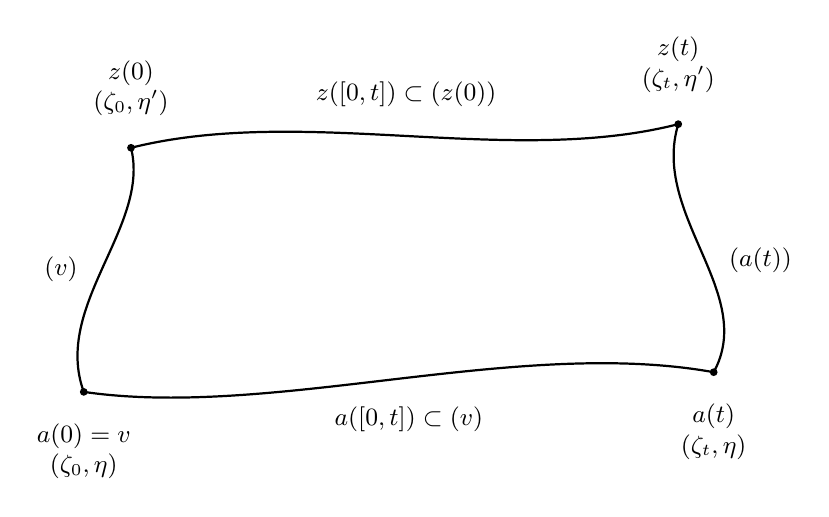
\begin{tikzpicture}[x=1cm,y=1cm,font=\small]
  \coordinate (v) at (0,0);
  \coordinate (a) at (8,0.25);
  \coordinate (z0) at (0.6,3.1);
  \coordinate (zt) at (7.55,3.4);
  \draw[thick] (v) .. controls (2.4,-0.35) and (5.5,0.7) .. (a)
    node[pos=0.52,below=7pt] {$a([0,t])\subset\Ws(v)$};
  \draw[thick] (z0) .. controls (2.8,3.65) and (5.4,2.85) .. (zt)
    node[pos=0.50,above=7pt] {$z([0,t])\subset\Ws(z(0))$};
  \draw[thick] (v) .. controls (-0.4,1.1) and (0.85,2.1) .. (z0)
    node[pos=0.49,left=5pt] {$\Wu(v)$};
  \draw[thick] (a) .. controls (8.55,1.25) and (7.2,2.25) .. (zt)
    node[pos=0.47,right=5pt] {$\Wu(a(t))$};
  \fill (v) circle (1.4pt);
  \fill (a) circle (1.4pt);
  \fill (z0) circle (1.4pt);
  \fill (zt) circle (1.4pt);
  \node[below=8pt,align=center] at (v)
    {$a(0)=v$\\$ (\zeta_0,\eta)$};
  \node[below=8pt,align=center] at (a)
    {$a(t)$\\$ (\zeta_t,\eta)$};
  \node[above=8pt,align=center] at (z0)
    {$z(0)$\\$ (\zeta_0,\eta')$};
  \node[above=8pt,align=center] at (zt)
    {$z(t)$\\$ (\zeta_t,\eta')$};
\end{tikzpicture}
\caption{Actual leaf incidences in the infinite-dimensional alternative,
for a fixed finite $t$. Each ordered pair gives the past and future
endpoints. The lower path is tangent to $P^s$; the translated upper
path is proved tangent to $E^s$. Each vertical connection indicates
membership in one strong unstable leaf. The drawing is schematic:
it asserts no ambient affine plane, smooth product chart or embedded
surface. The contradiction uses the proper lower ray and the endpoint
identities, not any geometric shape of this drawing.}
\label{fig:mixed-rectangle}
\end{figure}


We claim
\begin{equation}\label{real:busemann-divergence}
 b_{\zeta_t}(a(t))\longrightarrow-\infty.
\end{equation}
The sum $b_\eta+b_{\zeta_t}$ is convex and has zero gradient on
the geodesic with these endpoints, so it attains its minimum
there. Let $c(r)$ be the ray from $o$ toward $\eta$. For each
fixed $r>0$,
\[
 b_\eta(a(t))+b_{\zeta_t}(a(t))
      \le b_\eta(c(r))+b_{\zeta_t}(c(r)).
\]
As $t\to\infty$ the right-hand side tends to $-2r$, by endpoint
continuity of normalized Busemann functions. The term
$b_\eta(a(t))=b_\eta(v)$ is fixed. Since $r$ is arbitrary,
\eqref{real:busemann-divergence} follows.

On the other hand, $z(t)$ has ordered endpoints
$(\zeta_t,\eta')$ and fixed future Busemann level
$b_{\eta'}(z(0))$. Their limiting pair $(\eta,\eta')$ is off the
diagonal. The corresponding unit tangent vectors therefore
converge to the vector with this limiting pair and that level;
in particular they remain in a compact subset of
$S\widetilde M$. Endpoint continuity now makes
$b_{\zeta_t}(z(t))$ bounded. But $z(t)\in\Wu(a(t))$ means that
the two vectors have the same past endpoint and past Busemann
level, so
\[
 b_{\zeta_t}(z(t))=b_{\zeta_t}(a(t)).
\]
This contradicts \eqref{real:busemann-divergence} and excludes
the infinite-dimensional alternative.
\end{proof}
